%-------------------------------
%	DOCUMENT SETTINGS
%-------------------------------
\documentclass[a4paper]{article}

\setlength{\hoffset}{-3.2cm}
\setlength{\voffset}{-3cm}
\setlength{\textwidth}{18.7cm}
\setlength{\textheight}{25.5cm}
\setlength{\parskip}{0pt}
\setlength{\parindent}{0in}

%----------------------------------------------------------------------------------------
%	PACKAGES AND OTHER DOCUMENT CONFIGURATIONS
%----------------------------------------------------------------------------------------

\usepackage{mathtools}
\usepackage{dsfont}
\usepackage[shortlabels]{enumitem}
\DeclarePairedDelimiter\abs{\lvert}{\rvert}%
\usepackage{cancel}
\usepackage{blindtext} % Package to generate dummy text
\usepackage{charter} % Use the Charter font
\usepackage[utf8]{inputenc} % Use UTF-8 encoding
\usepackage{microtype} % Slightly tweak font spacing for aesthetics
\usepackage[english]{babel} % Language hyphenation and typographical rules
\usepackage{amsthm, amsmath, amssymb} % Mathematical typesetting
\usepackage{float} % Improved interface for floating objects
\usepackage[final, colorlinks = true, 
linkcolor = black, 
citecolor = black]{hyperref} % For hyperlinks in the PDF
\usepackage{graphicx, multicol} % Enhanced support for graphics
\usepackage{xcolor} % Driver-independent color extensions
\usepackage{marvosym, wasysym} % More symbols
\usepackage{rotating} % Rotation tools
\usepackage{censor} % Facilities for controlling restricted text
\usepackage{listings} % Environment for non-formatted code, !uses style file!
\usepackage{pseudocode} % Environment for specifying algorithms in a natural way
% Environment for f-structures, !uses style file!
\usepackage{booktabs} % Enhances quality of tables
\usepackage{tikz-qtree} % Easy tree drawing tool
% Configuration for b-trees and b+-trees, !uses style file!
%\usepackage[backend=biber,style=numeric,
%            sorting=nyt]{biblatex} % Complete reimplementation of bibliographic facilities
%\addbibresource{ecl.bib}
\usepackage{csquotes} % Context sensitive quotation facilities
\usepackage[yyyymmdd]{datetime} % Uses YEAR-MONTH-DAY format for dates
\renewcommand{\dateseparator}{-} % Sets dateseparator to '-'
\usepackage{fancyhdr} % Headers and footers
\pagestyle{fancy} % All pages have headers and footers
\fancyhead{}\renewcommand{\headrulewidth}{0pt} % Blank out the default header
\fancyfoot[L]{} % Custom footer text
\fancyfoot[C]{} % Custom footer text
\fancyfoot[R]{\thepage} % Custom footer text
\newcommand{\note}[1]{\marginpar{\scriptsize \textcolor{red}{#1}}} % Enables comments in red on margin

%----------------------------------------------------------------------------------------
%	GENERATED BY RSTUDIO
%----------------------------------------------------------------------------------------

\usepackage{lmodern}
\usepackage{amssymb,amsmath}
\usepackage{ifxetex,ifluatex}
\ifnum 0\ifxetex 1\fi\ifluatex 1\fi=0 % if pdftex
\usepackage[T1]{fontenc}
\usepackage[utf8]{inputenc}
\usepackage{textcomp} % provide euro and other symbols
\else % if luatex or xetex
\usepackage{unicode-math}
\defaultfontfeatures{Scale=MatchLowercase}
\defaultfontfeatures[\rmfamily]{Ligatures=TeX,Scale=1}
\fi

% Use upquote if available, for straight quotes in verbatim environments
\IfFileExists{upquote.sty}{\usepackage{upquote}}{}
\IfFileExists{microtype.sty}{% use microtype if available
	\usepackage[]{microtype}
	\UseMicrotypeSet[protrusion]{basicmath} % disable protrusion for tt fonts
}{}

\makeatletter
\@ifundefined{KOMAClassName}{% if non-KOMA class
	\IfFileExists{parskip.sty}{%
		\usepackage{parskip}
	}{% else
		\setlength{\parindent}{0pt}
		\setlength{\parskip}{6pt plus 2pt minus 1pt}}
}{% if KOMA class
	\KOMAoptions{parskip=half}}


\makeatother
\usepackage{xcolor}
\IfFileExists{xurl.sty}{\usepackage{xurl}}{} % add URL line breaks if available
\IfFileExists{bookmark.sty}{\usepackage{bookmark}}{\usepackage{hyperref}}
\urlstyle{same} % disable monospaced font for URLs
\usepackage{color}
\usepackage{fancyvrb}
\newcommand{\VerbBar}{|}
\newcommand{\VERB}{\Verb[commandchars=\\\{\}]}
\DefineVerbatimEnvironment{Highlighting}{Verbatim}{commandchars=\\\{\}}
% Add ',fontsize=\small' for more characters per line

\usepackage{framed}
\definecolor{shadecolor}{RGB}{248,248,248}
\newenvironment{Shaded}{\begin{snugshade}}{\end{snugshade}}
\newcommand{\AlertTok}[1]{\textcolor[rgb]{0.94,0.16,0.16}{#1}}
\newcommand{\AnnotationTok}[1]{\textcolor[rgb]{0.56,0.35,0.01}{\textbf{\textit{#1}}}}
\newcommand{\AttributeTok}[1]{\textcolor[rgb]{0.77,0.63,0.00}{#1}}
\newcommand{\BaseNTok}[1]{\textcolor[rgb]{0.00,0.00,0.81}{#1}}
\newcommand{\BuiltInTok}[1]{#1}
\newcommand{\CharTok}[1]{\textcolor[rgb]{0.31,0.60,0.02}{#1}}
\newcommand{\CommentTok}[1]{\textcolor[rgb]{0.56,0.35,0.01}{\textit{#1}}}
\newcommand{\CommentVarTok}[1]{\textcolor[rgb]{0.56,0.35,0.01}{\textbf{\textit{#1}}}}
\newcommand{\ConstantTok}[1]{\textcolor[rgb]{0.00,0.00,0.00}{#1}}
\newcommand{\ControlFlowTok}[1]{\textcolor[rgb]{0.13,0.29,0.53}{\textbf{#1}}}
\newcommand{\DataTypeTok}[1]{\textcolor[rgb]{0.13,0.29,0.53}{#1}}
\newcommand{\DecValTok}[1]{\textcolor[rgb]{0.00,0.00,0.81}{#1}}
\newcommand{\DocumentationTok}[1]{\textcolor[rgb]{0.56,0.35,0.01}{\textbf{\textit{#1}}}}
\newcommand{\ErrorTok}[1]{\textcolor[rgb]{0.64,0.00,0.00}{\textbf{#1}}}
\newcommand{\ExtensionTok}[1]{#1}
\newcommand{\FloatTok}[1]{\textcolor[rgb]{0.00,0.00,0.81}{#1}}
\newcommand{\FunctionTok}[1]{\textcolor[rgb]{0.00,0.00,0.00}{#1}}
\newcommand{\ImportTok}[1]{#1}
\newcommand{\InformationTok}[1]{\textcolor[rgb]{0.56,0.35,0.01}{\textbf{\textit{#1}}}}
\newcommand{\KeywordTok}[1]{\textcolor[rgb]{0.13,0.29,0.53}{\textbf{#1}}}
\newcommand{\NormalTok}[1]{#1}
\newcommand{\OperatorTok}[1]{\textcolor[rgb]{0.81,0.36,0.00}{\textbf{#1}}}
\newcommand{\OtherTok}[1]{\textcolor[rgb]{0.56,0.35,0.01}{#1}}
\newcommand{\PreprocessorTok}[1]{\textcolor[rgb]{0.56,0.35,0.01}{\textit{#1}}}
\newcommand{\RegionMarkerTok}[1]{#1}
\newcommand{\SpecialCharTok}[1]{\textcolor[rgb]{0.00,0.00,0.00}{#1}}
\newcommand{\SpecialStringTok}[1]{\textcolor[rgb]{0.31,0.60,0.02}{#1}}
\newcommand{\StringTok}[1]{\textcolor[rgb]{0.31,0.60,0.02}{#1}}
\newcommand{\VariableTok}[1]{\textcolor[rgb]{0.00,0.00,0.00}{#1}}
\newcommand{\VerbatimStringTok}[1]{\textcolor[rgb]{0.31,0.60,0.02}{#1}}
\newcommand{\WarningTok}[1]{\textcolor[rgb]{0.56,0.35,0.01}{\textbf{\textit{#1}}}}
\usepackage{graphicx,grffile}
\makeatletter
\def\maxwidth{\ifdim\Gin@nat@width>\linewidth\linewidth\else\Gin@nat@width\fi}
\def\maxheight{\ifdim\Gin@nat@height>\textheight\textheight\else\Gin@nat@height\fi}
\makeatother
% Scale images if necessary, so that they will not overflow the page
% margins by default, and it is still possible to overwrite the defaults
% using explicit options in \includegraphics[width, height, ...]{}
\setkeys{Gin}{width=\maxwidth,height=\maxheight,keepaspectratio}
% Set default figure placement to htbp
\makeatletter
\def\fps@figure{htbp}
\makeatother
\setlength{\emergencystretch}{3em} % prevent overfull lines
\providecommand{\tightlist}{%
	\setlength{\itemsep}{0pt}\setlength{\parskip}{0pt}}
\setcounter{secnumdepth}{-\maxdimen} % remove section numbering

%----------------------------------------------------------------------------------------
%	CUSTOM COMMANDS
%----------------------------------------------------------------------------------------

\newcommand{\R}{\mathbb{R}}
\newcommand{\E}{\mathbb{E}}
\newcommand{\I}{\mathbb{I}}
\newcommand{\Var}{\text{Var}}
% Para poner sonrisa sobre puntos suspensivos. Uso: \overplace{n}{\dotsc}
\newcommand{\overplace}[2]{%
	\overset{\substack{#1\\\smile}}{#2}%
}

\begin{document}
	
%-------------------------------
%	TITLE SECTION
%-------------------------------

\fancyhead[C]{}
\hrule \medskip % Upper rule
\begin{minipage}{0.295\textwidth} 
	\raggedright
	\footnotesize
	José Antonio Álvarez Ocete \hfill\\   
	77553417Q \hfill\\
	joseantonio.alvarezo@estudiante.uam.es
\end{minipage}
\begin{minipage}{0.4\textwidth} 
	\centering 
	\large 
	Entrega de problemas Boostrap\\ 
	\normalsize 
	Métodos Avanzados en Estadística\\ 
\end{minipage}
\begin{minipage}{0.295\textwidth} 
	\raggedleft
	\today\hfill\\
\end{minipage}
\medskip\hrule 
\bigskip

%-------------------------------
%	CONTENTS
%-------------------------------

\section*{Ejercicio 6.}

\textbf{Enunciado.} Sean $X_1, \ldots, X_n$ variables aleatorias \emph{i.i.d.} de una distribución con densidad $f$. Se considera el estimador del núcleo $\hat f$ con núcleo rectangular $K(x) = \I_{[-1/2,1/2]}(x)$ y parámetro de suavizado $h$.

\begin{enumerate}[a)]
	\item Calcula el sesgo y la varianza de $\hat f(x)$, para un valor de $x$ fijo.
	
	\item Demuestra que tanto el sesgo como la varianza tienden a cero si $h \rightarrow 0$ y $nh \rightarrow \infty$.
\end{enumerate}

Al estudiar el sesgo y la varianza de $\hat f(x)$ para un valor de $x$ fijo, estudiamos dichos valores respecto a la muestra tomada de  $X_1, \ldots, X_n$. En primer lugar, calculemos la esperanza del núcleo rectangular dado por la función indicatriz:

\[
	\E \bigg[ K\bigg(\frac{x - t}{h}\bigg) \bigg] = \int_{-\infty}^{+\infty} f(t) \; K\bigg(\frac{x - t}{h}\bigg) \; \text{t}w 
\]

Utilizamos el cambio de variable $w = \frac{x-t}{h}, \text = -\frac{dt}{h}$ e invirtiendo los límites de integración obtenemos:

\begin{align}
	\label{eq-nucleo}
	\begin{split}
		\E \bigg[ K\bigg(\frac{x - t}{h}\bigg) \bigg] & = \int_{-\infty}^{+\infty} f(t) \; K\bigg(\frac{x - t}{h}\bigg) \; \text{t}w \\
		& = \int_{+\infty}^{-\infty} f(x - wh) \; K(w) \; (-h) \; \text{d}w \\
		& = h \int_{-\infty}^{+\infty} f(x - wh) \; \I_{[-1/2,1/2]}(w) \; \text{d}w \\
		& = h \int_{-\frac{1}{2}}^{\frac{1}{2}} f(x - wh) \text{d}w \\
	\end{split}
\end{align}

Calculemos el sesgo de nuestro estimador del núcleo haciendo uso de la expresión anterior. Para ello calculamos su esperanza:

\begin{align*}
	\E [ \hat f(x)] & = \E \bigg[ \frac{1}{nh} \sum_{i=1}^n K\bigg(\frac{x - t}{h}\bigg) \bigg] \\
	& \stackrel{\text{iid}}{=} \frac{1}{nh} \; n \E \bigg[ K\bigg(\frac{x - t}{h}\bigg) \bigg] \\
	& \stackrel{(\ref{eq-nucleo})}{=} \frac{1}{h} \; h \int_{-\frac{1}{2}}^{\frac{1}{2}} f(x - wh) \text{d}w \\
	& = \int_{-\frac{1}{2}}^{\frac{1}{2}} f(x - wh) \text{d}w \\
\end{align*}

Este valor únicamente depende del punto fijado $x$, el parámetro de suavizado $h$ y la función de densidad $f$. Su valor equivale al área bajo la gráfica de $f$ en el intervalo $[x - h/2, x + h/2]$, como se puede apreciar en la figura \ref{fig-sesgo}. \\

\begin{figure}[H]
	\centering
	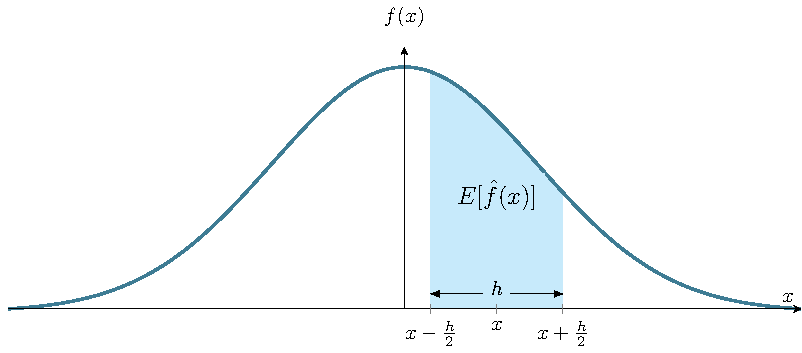
\includegraphics[width=17cm]{figures/sesgo}
	\caption{Representación gráfica del valor $\E [\hat f(x)]$.}
	\label{fig-sesgo}
\end{figure}

Es decir, estamos aproximando el valor de una función en un punto por su integral en un intervalor centrado en dicho punto. Naturalmente, al tomar $h \rightarrow 0$, dicho valor tiende al valor del punto. Es decir, el sesgo tiende a $0$. Analíticamente:

\begin{align*}
	\text{Sesgo}(f) & = E [ \hat f(x) ] - f(x) \\
	& = \int_{-\frac{1}{2}}^{\frac{1}{2}} f(x - wh) \text{d}w - f(x) \\
	& \stackrel{h \rightarrow \infty}{\longrightarrow} \int_{-\frac{1}{2}}^{\frac{1}{2}} f(x) \text{d}w - f(x) \\
	& =  f(x) \underbrace{\int_{-\frac{1}{2}}^{\frac{1}{2}} \text{d}w}_{= 1} - f(x) \\
	& =  f(x) - f(x) = 0 \\
\end{align*}

Por otro lado, podemos darnos cuenta de lo siguiente:

\begin{equation}
	\label{eq-cuadrado}
	K(x)^2 = K(x) \quad \forall x \in \R,
\end{equation}

pues la función indicatriz tiene por imagen el conjunto $\{0,1\}$ y la función $x \mapsto x^2$ sobre este conjunto es la identidad. Calculemos la varianza del estimador del núcleo:

\begin{align*}
	\Var [ \hat f(x)] & = \Var \bigg[ \frac{1}{nh} \sum_{i=1}^n K\bigg(\frac{x - t}{h}\bigg) \bigg] \\
	& \stackrel{\text{iid}}{=} \frac{1}{n^2 h^2} \; n \Var \bigg[ K\bigg(\frac{x - t}{h}\bigg) \bigg] \\
	& = \frac{1}{n h^2} \bigg( \E \bigg[ K\bigg(\frac{x - t}{h}\bigg)^2 \bigg] - \E \bigg[ K\bigg(\frac{x - t}{h}\bigg) \bigg]^2 \bigg)  \\
	& \stackrel{(\ref{eq-cuadrado})}{=} \frac{1}{n h^2} \bigg( \E \bigg[ K\bigg(\frac{x - t}{h}\bigg) \bigg] - \E \bigg[ K\bigg(\frac{x - t}{h}\bigg) \bigg]^2 \bigg)  \\
	& \stackrel{(\ref{eq-nucleo})}{=} \frac{1}{n h^2} \bigg( h \; \int_{-\frac{1}{2}}^{\frac{1}{2}} f(x - wh) \text{d}w - h^2 \; \bigg( \int_{-\frac{1}{2}}^{\frac{1}{2}} f(x - wh) \text{d}w\bigg) ^2 \bigg) \\
	& = \frac{1}{n h} \bigg( \int_{-\frac{1}{2}}^{\frac{1}{2}} f(x - wh) \text{d}w - h \; \bigg( \int_{-\frac{1}{2}}^{\frac{1}{2}} f(x - wh) \text{d}w\bigg) ^2 \bigg) \\
\end{align*}

Finalmente probamos que la varianza tiende a $0$ si $h \rightarrow 0$ y $nh \rightarrow \infty$:

\[
	\Var [ \hat f(x)] = \underbrace{\frac{1}{n h}}_{\hookrightarrow 0} \bigg( \underbrace{\int_{-\frac{1}{2}}^{\frac{1}{2}} f(x - wh) \text{d}w}_{\hookrightarrow f(x)} - \underbrace{h \; \bigg( \int_{-\frac{1}{2}}^{\frac{1}{2}} f(x - wh) \text{d}w\bigg) ^2}_{\hookrightarrow 0} \bigg)
	\longrightarrow 0
\]

Aunque ya probamos que el error cuadrático medio para un núcleo cualquiera tiende a $0$, en este ejercicio lo hemos probado para el caso del núcleo indicatriz sin el uso de aproximaciones.

\section*{Ejercicio 7.}

\textbf{Enunciado.} Considera una variable aleatoria con distribución beta de parámetros $\alpha = 3$, $\beta = 6$.

\begin{enumerate}[a)]
	\item Representa gráficamente la función de densidad y la función de distribución.

	Importamos los paquetes necesarios:

\begin{Shaded}
\begin{Highlighting}[]
\KeywordTok{library}\NormalTok{(tidyverse)}
\KeywordTok{library}\NormalTok{(gapminder)}
\KeywordTok{library}\NormalTok{(comprehenr)}
\KeywordTok{library}\NormalTok{(ggplot2)}
\KeywordTok{library}\NormalTok{(dplyr)}
\KeywordTok{library}\NormalTok{(ggpubr)}

\NormalTok{defaultW <-}\StringTok{ }\KeywordTok{getOption}\NormalTok{(}\StringTok{"warn"}\NormalTok{)}
\KeywordTok{options}\NormalTok{(}\DataTypeTok{warn =} \DecValTok{-1}\NormalTok{)}
\KeywordTok{theme_set}\NormalTok{(}\KeywordTok{theme_bw}\NormalTok{())}
\end{Highlighting}
\end{Shaded}

	Representamos las funciones especificadas:

\begin{Shaded}
\begin{Highlighting}[]
\NormalTok{x =}\StringTok{ }\KeywordTok{seq}\NormalTok{(}\DecValTok{0}\NormalTok{, }\DecValTok{1}\NormalTok{, }\DataTypeTok{length=}\DecValTok{1000}\NormalTok{)}
\NormalTok{pdf =}\StringTok{ }\KeywordTok{dbeta}\NormalTok{(x, }\DecValTok{3}\NormalTok{, }\DecValTok{6}\NormalTok{)}
\NormalTok{cdf =}\StringTok{ }\KeywordTok{pbeta}\NormalTok{(x, }\DecValTok{3}\NormalTok{, }\DecValTok{6}\NormalTok{)}
\NormalTok{df <-}\StringTok{ }\KeywordTok{data.frame}\NormalTok{(x, pdf, cdf)}

\NormalTok{graf1 <-}\StringTok{ }\KeywordTok{ggplot}\NormalTok{(df, }\KeywordTok{aes}\NormalTok{(}\DataTypeTok{x=}\NormalTok{x, }\DataTypeTok{y=}\NormalTok{pdf)) }\OperatorTok{+}
\StringTok{  }\KeywordTok{geom_ribbon}\NormalTok{(}\KeywordTok{aes}\NormalTok{(}\DataTypeTok{ymin=}\DecValTok{0}\NormalTok{, }\DataTypeTok{ymax=}\NormalTok{pdf), }\DataTypeTok{fill=}\StringTok{"lightblue"}\NormalTok{, }\DataTypeTok{col=}\StringTok{"blue"}\NormalTok{, }\DataTypeTok{alpha=}\FloatTok{0.5}\NormalTok{) }\OperatorTok{+}
\StringTok{  }\KeywordTok{ylab}\NormalTok{(}\StringTok{"Probability  Function"}\NormalTok{)}

\NormalTok{graf2 <-}\StringTok{ }\KeywordTok{ggplot}\NormalTok{(df, }\KeywordTok{aes}\NormalTok{(}\DataTypeTok{x=}\NormalTok{x, }\DataTypeTok{y=}\NormalTok{cdf)) }\OperatorTok{+}
\StringTok{  }\KeywordTok{geom_ribbon}\NormalTok{(}\KeywordTok{aes}\NormalTok{(}\DataTypeTok{ymin=}\DecValTok{0}\NormalTok{, }\DataTypeTok{ymax=}\NormalTok{cdf), }\DataTypeTok{fill=}\StringTok{"lightblue"}\NormalTok{, }\DataTypeTok{col=}\StringTok{"blue"}\NormalTok{, }\DataTypeTok{alpha=}\FloatTok{0.5}\NormalTok{) }\OperatorTok{+}
\StringTok{  }\KeywordTok{ylab}\NormalTok{(}\StringTok{"Cumulative Density Function"}\NormalTok{)}

\KeywordTok{ggarrange}\NormalTok{(graf1, graf2, }
\DataTypeTok{ncol =} \DecValTok{2}\NormalTok{, }\DataTypeTok{nrow =} \DecValTok{1}\NormalTok{)}
\end{Highlighting}
\end{Shaded}

	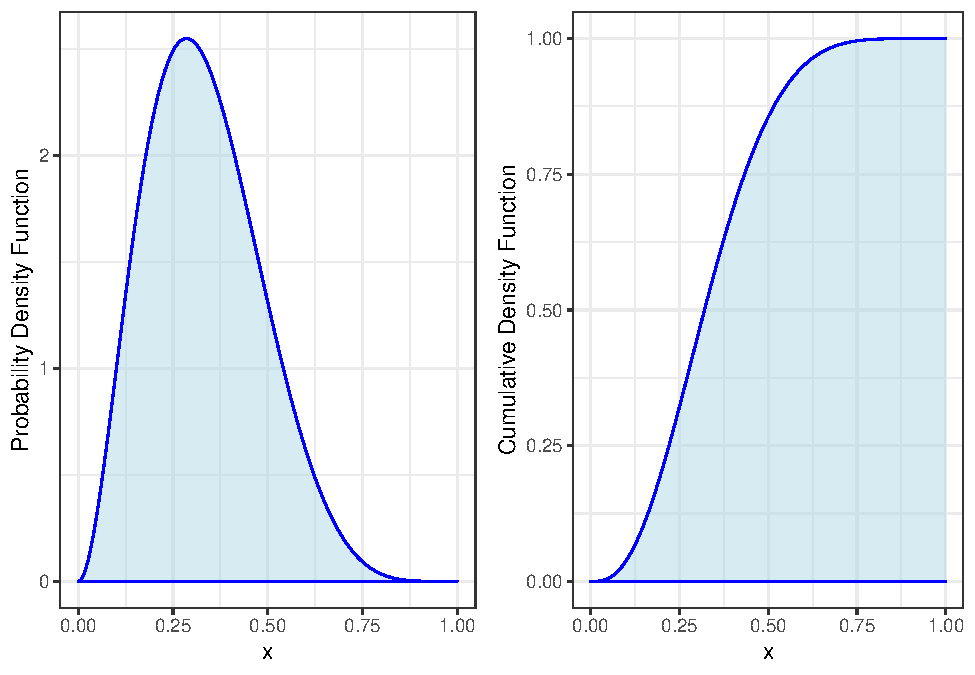
\includegraphics{figures/7a}
	
	\item Simula una muestra de tamaño $20$ de esta distribución. A continuación, representa en los
	mismos gráficos del apartado (a) las estimaciones de $F$ y $f$ obtenidas respectivamente
	mediante la función de distribución empírica $F_n$ y un estimador del núcleo $\hat f$ obtenidos
	a partir de la muestra simulada.
	
	Para este apartado, generamos una muestra del tamaño especificado y estimamos las funciones de densidad generando un estimador del núcleo utilizando el comando de R \KeywordTok{density}. Pintamos ambas estimaciones sobre las gráficas anteriores para poder comprobar los resultados.
	
\begin{Shaded}
\begin{Highlighting}[]
\KeywordTok{set.seed}\NormalTok{(}\DecValTok{123}\NormalTok{)}

\NormalTok{x =}\StringTok{ }\KeywordTok{seq}\NormalTok{(}\DecValTok{0}\NormalTok{, }\DecValTok{1}\NormalTok{, }\DataTypeTok{length=}\DecValTok{1000}\NormalTok{)}
\NormalTok{pdf =}\StringTok{ }\KeywordTok{dbeta}\NormalTok{(x, }\DecValTok{3}\NormalTok{, }\DecValTok{6}\NormalTok{)}
\NormalTok{cdf =}\StringTok{ }\KeywordTok{pbeta}\NormalTok{(x, }\DecValTok{3}\NormalTok{, }\DecValTok{6}\NormalTok{)}
\NormalTok{df <-}\StringTok{ }\KeywordTok{data.frame}\NormalTok{(x, pdf, cdf)}

\NormalTok{muestra <-}\StringTok{ }\KeywordTok{rbeta}\NormalTok{(}\DecValTok{20}\NormalTok{, }\DecValTok{3}\NormalTok{, }\DecValTok{6}\NormalTok{)}
\NormalTok{estimador_nucleo <-}\StringTok{ }\KeywordTok{density}\NormalTok{(muestra)}
\NormalTok{df_estimator <-}\StringTok{ }\KeywordTok{data.frame}\NormalTok{(}\StringTok{"x"}\NormalTok{=estimador_nucleo}\OperatorTok{$}\NormalTok{x, }\StringTok{"y"}\NormalTok{=estimador_nucleo}\OperatorTok{$}\NormalTok{y)}

\NormalTok{graf1 <-}\StringTok{ }\KeywordTok{ggplot}\NormalTok{() }\OperatorTok{+}
\StringTok{  }\KeywordTok{geom_ribbon}\NormalTok{(}\DataTypeTok{data=}\NormalTok{df, }\KeywordTok{aes}\NormalTok{(}\DataTypeTok{x=}\NormalTok{x, }\DataTypeTok{y=}\NormalTok{pdf, }\DataTypeTok{ymin=}\DecValTok{0}\NormalTok{, }\DataTypeTok{ymax=}\NormalTok{pdf),}
\DataTypeTok{fill=}\StringTok{"lightblue"}\NormalTok{, }\DataTypeTok{col=}\StringTok{"blue"}\NormalTok{, }\DataTypeTok{alpha=}\FloatTok{0.5}\NormalTok{) }\OperatorTok{+}
\StringTok{  }\KeywordTok{geom_line}\NormalTok{(}\DataTypeTok{data=}\NormalTok{df_estimator, }\KeywordTok{aes}\NormalTok{(}\DataTypeTok{x=}\NormalTok{x, }\DataTypeTok{y=}\NormalTok{y), }\DataTypeTok{col=}\StringTok{"red"}\NormalTok{) }\OperatorTok{+}
\StringTok{  }\KeywordTok{ylab}\NormalTok{(}\StringTok{"Probability Density Function"}\NormalTok{) }\OperatorTok{+}
\StringTok{  }\KeywordTok{coord_cartesian}\NormalTok{(}\DataTypeTok{xlim =} \KeywordTok{c}\NormalTok{(}\DecValTok{0}\NormalTok{, }\DecValTok{1}\NormalTok{))}

\NormalTok{graf2 <-}\StringTok{ }\KeywordTok{ggplot}\NormalTok{() }\OperatorTok{+}
\StringTok{  }\KeywordTok{geom_ribbon}\NormalTok{(}\DataTypeTok{data=}\NormalTok{df, }\KeywordTok{aes}\NormalTok{(}\DataTypeTok{x=}\NormalTok{x, }\DataTypeTok{y=}\NormalTok{cdf, }\DataTypeTok{ymin=}\DecValTok{0}\NormalTok{, }\DataTypeTok{ymax=}\NormalTok{cdf),}
\DataTypeTok{fill=}\StringTok{"lightblue"}\NormalTok{, }\DataTypeTok{col=}\StringTok{"blue"}\NormalTok{, }\DataTypeTok{alpha=}\FloatTok{0.5}\NormalTok{) }\OperatorTok{+}
\StringTok{  }\KeywordTok{stat_ecdf}\NormalTok{(}\DataTypeTok{data=}\KeywordTok{data.frame}\NormalTok{(muestra), }\KeywordTok{aes}\NormalTok{(}\DataTypeTok{x=}\NormalTok{muestra), }\DataTypeTok{color=}\StringTok{"red"}\NormalTok{, }\DataTypeTok{geom=}\StringTok{"step"}\NormalTok{) }\OperatorTok{+}
\StringTok{  }\KeywordTok{ylab}\NormalTok{(}\StringTok{"Cumulative Density Function"}\NormalTok{) }\OperatorTok{+}
\StringTok{  }\KeywordTok{coord_cartesian}\NormalTok{(}\DataTypeTok{xlim =} \KeywordTok{c}\NormalTok{(}\DecValTok{0}\NormalTok{, }\DecValTok{1}\NormalTok{))}

\KeywordTok{ggarrange}\NormalTok{(graf1, graf2, }\DataTypeTok{ncol =} \DecValTok{2}\NormalTok{, }\DataTypeTok{nrow =} \DecValTok{1}\NormalTok{)}
\end{Highlighting}
\end{Shaded}

	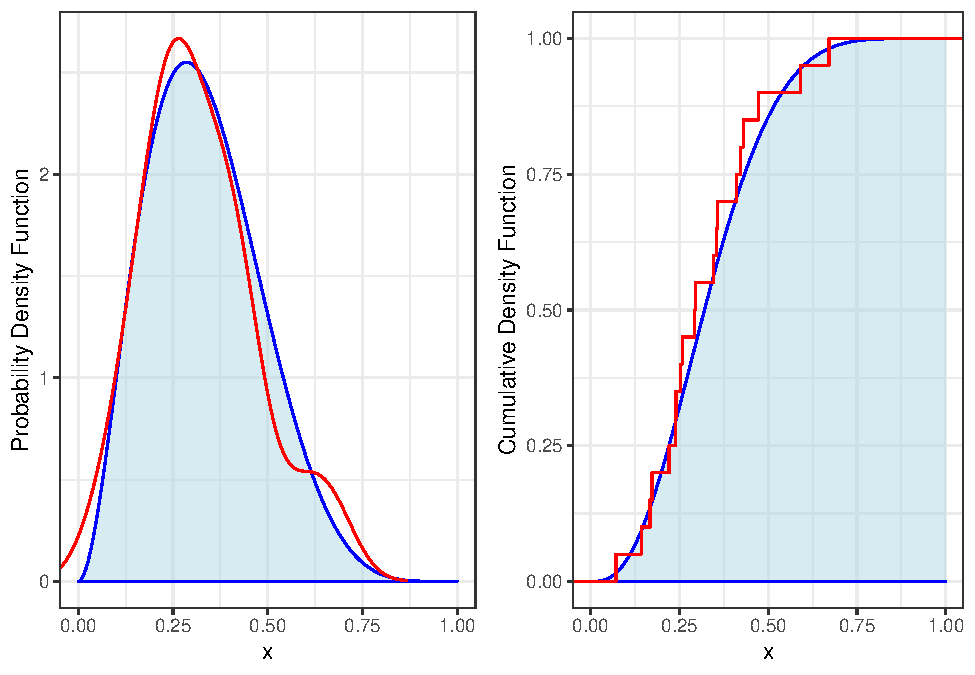
\includegraphics{figures/7b}
	
	Como podemos apreciar, ambas funciones son notablemente parecidas a las objetivo. Sin embargo, no se obtienen valores de estas aproximaciones tan buenos para todas las semillas. Basta con relanzar el experimento con otra semilla y comparar los resultados para apreciarlo.
	
	\item Verifica empíricamente el grado de aproximación alcanzado en las estimaciones de $F$
	y $f$. Para ello, genera $200$ muestras de tamaño $20$ y para cada una de ellas evalúa el
	error (medido en la norma del supremo, es decir, el máximo de las diferencias entre las
	funciones) cometido al aproximar $F$ por $F_n$ y $f$ por $\hat f$. Por último, calcula el promedio
	de los $200$ errores obtenidos.
	
	

\begin{Shaded}
\begin{Highlighting}[]
\KeywordTok{set.seed}\NormalTok{(}\DecValTok{123}\NormalTok{)}

\NormalTok{n <-}\StringTok{ }\DecValTok{20}
\NormalTok{m <-}\StringTok{ }\DecValTok{200}
\NormalTok{alpha <-}\StringTok{ }\DecValTok{3}
\NormalTok{beta <-}\StringTok{ }\DecValTok{6}

\NormalTok{errors_pdf <-}\StringTok{ }\OtherTok{NULL}
\NormalTok{errors_cdf <-}\StringTok{ }\OtherTok{NULL}
\NormalTok{p_values_pdf <-}\StringTok{ }\OtherTok{NULL}
\NormalTok{p_values_cdf <-}\StringTok{ }\OtherTok{NULL}

\ControlFlowTok{for}\NormalTok{ (i }\ControlFlowTok{in} \DecValTok{1}\OperatorTok{:}\NormalTok{m)\{}
\NormalTok{  muestra <-}\StringTok{ }\KeywordTok{rbeta}\NormalTok{(n, alpha, beta)}

\NormalTok{  estimador_nucleo <-}\StringTok{ }\KeywordTok{density}\NormalTok{(muestra)}
\NormalTok{  theoric_pdf_ys <-}\StringTok{ }\KeywordTok{dbeta}\NormalTok{(estimador_nucleo}\OperatorTok{$}\NormalTok{x, alpha, beta)}
\NormalTok{  ks_pdf <-}\StringTok{ }\KeywordTok{ks.test}\NormalTok{(estimador_nucleo}\OperatorTok{$}\NormalTok{y, theoric_pdf_ys)}

\NormalTok{  ecdf_estimada <-}\StringTok{ }\KeywordTok{ecdf}\NormalTok{(muestra)}
\NormalTok{  theoric_cdf_ys <-}\StringTok{ }\KeywordTok{pbeta}\NormalTok{(muestra, alpha, beta)}
\NormalTok{  ks_cdf <-}\StringTok{ }\KeywordTok{ks.test}\NormalTok{(}\KeywordTok{ecdf_estimada}\NormalTok{(muestra), }\StringTok{"pbeta"}\NormalTok{, alpha, beta)}

\NormalTok{  errors_pdf <-}\StringTok{ }\KeywordTok{c}\NormalTok{(errors_pdf, ks_pdf}\OperatorTok{$}\NormalTok{statistic)}
\NormalTok{  p_values_pdf <-}\StringTok{ }\KeywordTok{c}\NormalTok{(p_values_pdf, ks_pdf}\OperatorTok{$}\NormalTok{p.value)}
\NormalTok{  errors_cdf <-}\StringTok{ }\KeywordTok{c}\NormalTok{(errors_cdf, ks_cdf}\OperatorTok{$}\NormalTok{statistic)}
\NormalTok{  p_values_cdf <-}\StringTok{ }\KeywordTok{c}\NormalTok{(errors_cdf, ks_cdf}\OperatorTok{$}\NormalTok{p.value)}
\NormalTok{\}}

\KeywordTok{cat}\NormalTok{(}\StringTok{"Mean error in cdf: "}\NormalTok{, }\KeywordTok{mean}\NormalTok{(errors_cdf), }\StringTok{"}\CharTok{\textbackslash{}n}\StringTok{"}\NormalTok{)}
\end{Highlighting}
\end{Shaded}

\begin{verbatim}
## Mean error in cdf:  0.4115441
\end{verbatim}

\begin{Shaded}
\begin{Highlighting}[]
\KeywordTok{cat}\NormalTok{(}\StringTok{"Mean p-value for cdf: "}\NormalTok{, }\KeywordTok{mean}\NormalTok{(p_values_cdf), }\StringTok{"}\CharTok{\textbackslash{}n}\StringTok{"}\NormalTok{)}
\end{Highlighting}
\end{Shaded}

\begin{verbatim}
## Mean p-value for cdf:  0.4095036
\end{verbatim}

\begin{Shaded}
\begin{Highlighting}[]
\KeywordTok{cat}\NormalTok{(}\StringTok{"Mean error in pdf: "}\NormalTok{, }\KeywordTok{mean}\NormalTok{(errors_pdf), }\StringTok{"}\CharTok{\textbackslash{}n}\StringTok{"}\NormalTok{)}
\end{Highlighting}
\end{Shaded}

\begin{verbatim}
## Mean error in pdf:  0.1869434
\end{verbatim}

\begin{Shaded}
\begin{Highlighting}[]
\KeywordTok{cat}\NormalTok{(}\StringTok{"Mean p-value for pdf: "}\NormalTok{, }\KeywordTok{mean}\NormalTok{(p_values_pdf), }\StringTok{"}\CharTok{\textbackslash{}n}\StringTok{"}\NormalTok{)}
\end{Highlighting}
\end{Shaded}

\begin{verbatim}
## Mean p-value for pdf:  0.0017868
\end{verbatim}


	
	
\end{enumerate}

\end{document}
